\documentclass[12pt]{article}
\usepackage[utf8]{inputenc}
\usepackage{fancyhdr}
\usepackage{graphicx}
\usepackage{geometry}
\usepackage{float}
\usepackage[utf8]{inputenc}
 
\usepackage{array}
\usepackage{makecell}

% ---- Commands ------- %
\newcommand{\documentNumber}[1]{
    \LARGE  \textbf{ Kravprocessbok }
    \\
    \medskip
}
\newcommand{\documentVersion}[1]{
    \medskip
}
\newcommand{\documentTitle}[1]{
    \centerline{\rule{13cm}{0.4pt}}
    \bigskip \bigskip
    \LARGE \textbf{Projekt IDA3} \\
    \bigskip
    \LARGE {#1} \\
    \bigskip \bigskip
    \centerline{\rule{13cm}{0.4pt}}
}

\newcommand{\documentDate}[1]{
    \date {#1} 
}

\renewcommand\theadalign{bc}
\renewcommand\theadfont{\bfseries}
\renewcommand\theadgape{\Gape[5pt]}
\renewcommand\cellgape{\Gape[5pt]}


\renewcommand{\contentsname}{Innehållsförtäckning}

% --- Header & Footer ---- %
\pagestyle{fancy}
\lhead{\leftmark}
\rhead{}
\rfoot{\thepage}
\cfoot{}
\lfoot{}


% ------------------------------------------------ #

% ----- FILL THIS ----- %
\title {
    \documentNumber {01}    

    % Full name - SHORTNAME
    \documentTitle {Helsingborg Event and Convention Bureau}
    
    % Format: YYYY-MM-DD
    \documentDate {2021-08-20}
    \documentVersion Vv 0.4
    
    \author{Anna Bergvall - Oscar Blixt - Pontus Persson - Filip Sjövall - David Vilppu}
}

\begin{document}
\addtocontents{toc}{\protect\setcounter{tocdepth}{2}}
\maketitle

\thispagestyle{empty}



\newpage

\tableofcontents


\newpage

\section{Dokument Historia}
\begin{tabular}{ l | l | l }
    Version & Date & Description \\
    \hline
    0.1 & 2021-09-12 & Dokumentet skapat.Loggbok V36, Övning 1 och 2 inlagda. \\
    \hline
    0.2 & 2021-09-20 & Loggbok V37, Övning 3 och 4 inlagda.
    \\
    \hline
    0.3 & 2021-09-27 & Loggbok V38 och Övning 5 inlagda.
    \\
    \hline
    0.4 & 2021-10-04 & Loggbok V39 inlagd.
     \\
    \hline
    0.5 & 2021-12-13 & Loggbok V48 och V49 inlagd.
    \\
\end{tabular}

\newpage

\section{Loggbok}
    \subsection{Vecka 36}
    \\
    Denna veckan har varit stort fokus på att komma igång. Det var första veckan vi träffades som grupp och pratade ihop oss om vad projektet kommer innebära. Arbetet har därför legat mer åt att organisera projektgruppen än kravhantering. \\ Varsitt möte med Malin Planander på Miljlbron samt Malin Hollgren, våran "kund" och två övningar inom kursen gav oss däremot en skjuts med att komma igång med kravarbetet, så under veckan har vi samlat på oss en del krav som nu måste konkritiseras och dokumenteras. 
    
    \subsection{Vecka 37}
    Denna veckan har fokus legat på att prata ihop oss med gruppen om de möten vi hade förra veckan, och utifrån dessa börja framställa krav. Vi har haft en del sjukdomar och medlemmar i gruppen som varit bortresta vilket gjort att vi ej kunnat ha några möten. Däremot har delgrupperna jobbat enskilt med övningarna och vi har kunnat kommunicera med varandra genom meddelanden.
    
    \subsection{Vecka 38}
    Denna veckan började vi med att strukturera upp kravspecifikationen utseende i form av rubriker, samt komma överens om arbetsfördelning inom delgrupperna. Vi har även framställt varsin prototyp av hemsidans utseende som vi diskuterat i gruppen. Utifrån dessa ska vi ta fram en mer omfattande designprototyp som skall visas upp för Malin Hollgren. Vi har även haft en fortsatt diskussion om dataserver och vilken vi ska använda. Detta måste vidarediskuteras med Malin. Övning fem gjordes inom delgrupperna och sammanställdes inom hela gruppen.
    
    \subsection{Vecka 39}
    Denna vecka har arbetet med krav lagts åt sidan för att arbeta mer med uppgifter inom projektet. Men tack vare det överlappande arbetet har även framsteg inom kravhantering gjorts. Vi i gruppen har bestämt oss för att jobba agilt med hjälp av Scrum-boards. Vi har därför börjat använda oss av hemsidan atlassian för att strukturera upp våran board. Med tanke på att vi kommer behöva experimentera med Scrum för att förfina arbetsmetoden så har vi än så länge inte bestämt mycket mer än att vi kommer använda oss av sprints som preliminärt kommer att ske i tvåveckors intervaller. 
    Med kravarbetet har vi valt att börja skriva in User stories som krav i våran scrumboard för att sedan referera hit i våran kravspecifikation. Detta för att underlätta så att krav inte finns på flera ställen samtidigt.
    Kommande vecka ska: \\ 
    \begin{itemize}
        \item Arbetet med strukturen av våran Scrumboard fortsätta.
        \item Möte med Malin Hollgren genomföras. Under mötet kommer flera 
        punkter klaras upp samt en disskusion föras för att komma fram till en mer slutgiltig design av hemsidan.
        \item våran första sprint börja där Er-diagram och UML-diagram skapas.
    \end{itemize}
    
    \subsection{Vecka 40}
    Under vecka 40 skickade vi in våra första design prototyper till Malin Hollgren, prototyperna bestod av sex stycken förslag där vi alla i gruppen hade gjort var sin prototyp. Lite ändringar gjordes sedan vecka 38 och vi bestämdes oss för att istället för att sammanställa en prototyp för att visa för Malin, så visas alla prototyper upp och efter mötet sammanställs istället en prototyp utifrån Malins synpunkter. \\
    \\
    På onsdagen hade vi sedan vårt första uppföljningsmöte med Malin där bland annat prototyperna diskuterades samt att vi klarade upp vissa frågor om design och frågor som handlade om hur användarna ska identifiera sig på hemsidan togs upp. I diskussionen om identifiering av användare kom Malin med förslag där hon ville att användarna skulle kunna identifiera sig via samma länk som de använder för att få tillgång till formuläret. Detta förlaget tog vi in men kom fram till att det inte går att genomföra med våra resurser och vi fortsatta spåna på en andra ideér där vi kom fram till att varje användare ska tilldelas en unik kod som de använder för att logga in i formuläret. \\
    \\
    Veckan fortsatte att vi skapade vårt första dokument för kravspecifikationen och avslutades med ett möte på fredagen där vi pratade om veckan som gått.
    
    \subsection{Vecka 41}
    I början av denna vecka hade vi ett arbetspass som sträckte sig hela dagen. Det var även under denna vecka vi påbörjade första sprinten, som vi beslutade skulle sträcka sig över en-veckorsperioder istället för två-veckorsperioder. Gruppen hade sedan tidigare bestämt att vi skulle bli klara med ER-diagram och UML-diagram. ER-diagramet blev klart och UML-diagramet bestämde vi oss för att slopa. Under arbetspasset sattes även en bas för all programmering upp, dvs. en html-fil kopplad till en utvecklingsserver som kommunicerar via Python. Vi diskuterade även att vi bör förtydliga för HASAB vad vi förväntar oss av dem. Vi skickade även en ny prototyp som skulle representera de egenskaper som Malin Hollgren tyckte om när vi presenterade ett flertal prototyper vecka 40. \\
    \\
    Eftersom vi hade ett så pass långt arbetspass under måndagen, hade vi endast ett mindre möte på fredagen där vi stämde av allt som gjordes, samt vad som ska ske under nästa sprint.
    
    \subsection{Vecka 42}
    Tentamensvecka, inget har hänt.
    
    \subsection{Vecka 43}
    Tentamensvecka, inget har hänt.
    
    \subsection{Vecka 44}
    Under den här veckan skulle ett första utkast av kravspecifikationen vara klart vilket gjorde att vårt kravarbete handlade om att sammanställa de kraven vi hade och föra in dessa i kravspecifikationen. För att göra specifikation mer tydlig och för att förlätta spårningen tog vi och numrerade om kraven från siffor(1.2.3) till bokstäver och siffror (R1). 
    \\
    Vi förde också in kraven från scrumboarden till specifikationen och fixade så att dessa motstsvarade varandra.
    \\
     Sedan tog vi tag i att börja spåna mer om vilka kvalitetskrav vi tyckte skulle passade in på produkten och en enkel prioritetslista togs fram för att se vilka kvalitetskrav vi skulle lägga mest tid på. Vi kom fram till att användbarhet, prestandad och säkerhet var de viktigaste delarna och utifrån dessa började vi spåna om krav. Vi tyckte det var svårt att veta hur vi skulle skriva kvalitetskrav, detta är en fråga vi kommer ta med oss till nästa veckas handledning. Vi sammanställde det vi kommit fram till och skickade in till Christin. 
    \subsection{Vecka 45}
 Denna vecka har fokus skiftat en del från dokumentskrivande till arbete med koden. Vi har implementerat samtliga HTML-sidor  samt fått upp en databas som kan kommunicera med hemsidan. Då python och flask är nytt för samtliga i gruppen har många timmar lagts på inläsning och långsamt utvecklande.   Utöver detta har vi haft handledning med kirre och gunther, handledning med Christin, uppföljningsmöte med våra handledare, samt projektcoachning med Ylva.  Vi har lagt märke till att våra handledare är benägna att ändra och lägga till krav efterhand som de dyker upp. Detta är något vi diskuterade  under handledningen med kirre och gunther. Där kom vi fram till att vi ska vara öppna för dessa nya krav men också hålla det som öppna krav. Detta är något vi tog till vara på och poängterade under uppföljningsmötet.  Under handledningen med Christin fick vi matnyttig feedback på kravspecifikationen som vi tog med oss när vi sedan jobbade med den under veckan. Vi kom fram till att vi endast behöve
Denna vecka har fokus skiftat en del från dokumentskrivande till arbete med koden. Vi har implementerat samtliga HTML-sidor 
samt fått upp en databas som kan kommunicera med hemsidan. Då python och flask är nytt för samtliga i gruppen har många timmar lagts på
inläsning och långsamt utvecklande. 
\\
\\
Utöver detta har vi haft handledning med kirre och gunther, handledning med Christin, uppföljningsmöte med våra handledare, samt projektcoachning med Ylva.
\\
\\
Vi har lagt märke till att våra handledare är benägna att ändra och lägga till krav efterhand som de dyker upp. Detta är något vi diskuterade 
under handledningen med kirre och gunther. Där kom vi fram till att vi ska vara öppna för dessa nya krav men också hålla det som öppna krav.
Detta är något vi tog till vara på och poängterade under uppföljningsmötet.
\\
\\
Under handledningen med Christin fick vi matnyttig feedback på kravspecifikationen som vi tog med oss när vi sedan jobbade med den under veckan.
Vi kom fram till att vi endast behöver ha med de kvalitetskrav som är viktigast och kan mätas. Det betyder att vi inte behöver fylla 
kravspecifikationen med överflödiga och underförstådda kvalitetskrav.
\\
\\
Under mötet med våra handledare kom vi fram till att vi ska ändra hur vi verifierar användarna. Istället för att använda en personlig kod verifierar vi användarna
med deras mejladress. Vi kom även fram till att vi inte kommer använda några frågor med fritext som svar. Detta på grund av att det försvårar statistikföringen
\\
\\
Denna vecka sammanställdes även en ny prototyp för adminsidan, denna visades för Malin och godkändes.
\\
\\
Överlag har det varit en produktiv vecka som fungerat lite som ett startskott efter en seg tentaperiod.
	\subsection{Vecka 46}
Denna veckan har vi mest jobbat med projektet, vilket innebär att det inte lagts särskilt mycket energi på kravarbetet. Däremot har vi börjat använda
oss av den grafiska mallen vi fått från Malin.
\\
\\
Utöver detta tog vi även ett gemensamt beslut att byta scrumboard till trello. Detta då vi anser att deras design är mer intuitiv vilket medför att
scrumboarden ses mer som ett verktyg än ett hinder.

\subsection{Vecka 47}
 Denna veckan har kravarbetet gått framåt och vi har börjat förbereda oss för slutgiltig inlämning av kravspecifikationen som skall lämnas in den tredje december. Vi håller på att diskutera fram leverans- och underhållskrav från Malin Hollgren och har än så länge kommit fram till att en i stort sätt slutgiltig produkt ska överlämnas den 13/12 som ska användas för testning hos HCEB. En genomgång av systemet ska även göras för att se om något behöver ändras eller anpassas.\\ När det kommer till hur underhållet av hemsidan så kan det bli så att funktionskrav kan tillkomma som gör att admin kan lägga till/ta bort frågor, vi är däremot inte säkra på om vi kommer kumma uppfylla dessa krav och har därför sagt att dessa tills vidare är sensationella krav. \\\\
 Under veckan har även enuppdaterad version av hemsidan tagits fram där utseendet av inmatning för användare har ändrats vilket också har lett till att vissa funktionskrav enklare har kunnat implementeras. \\\\
 Till nästa vecka ska vi fortsätta kravarbetet och färdigställa kravspecifikationen.
 \newpage
 \subsection{Vecka 48}
 Denna veckan har projektgruppen arbetat med att redigera kravspecifikationen utifrån den återkoppling Christin gav efter ett möte. Detta gjordes omgående och därmed kunde fokus läggas på övriga dokument och hemsidan. \\\\
 
 \subsection{Vecka 49}
 Eftersom projektgruppen var överens om att kravspecifikationen var färdigställd genomfördes endast ett par korrekturläsningar av dokumentet under denna vecka.
 
 

  
    \newpage
    
\section{Terminologi}
    \begin{enumerate}
        \item \textbf{Slutanvändare} - Användare inom supply chain som kommer rapportera in data i formuläret.
        
    \end{enumerate}
    

\section{Intressenter och elicitering v.36}

    \subsection{Nyckelintressenter}
        \begin{itemize}
            \item \textbf{Malin Hollberg, Helsingborg Convention and Event Bureau}.
                \\
            \item \textbf{Slutanvändarna}.
                \\
             \item \textbf{Utvecklarna av verktyget}. Vi som jobbar med projektet.
                \\
        \end{itemize}
        
    \subsection{Viktiga intressenter}
        \begin{itemize}
            \item \textbf{GDSM} - Global Destination Sustainability Movment. Företaget som tar hand om statistiken vårt system kommer att sammanställa.
             \\
            \item \textbf{Malin Planander, Miljöbron}.
            \\
            \item \textbf{Campus Helsingborg}. Våra handledare
        \end{itemize}
        
    \subsection{Mindre viktiga intressenter}
    \begin{itemize}
            \item \textbf{Företag som planerar event i Helsingborg}.
                \\
            \item \textbf{Robin Nilsson}. Verksamhetsledare på Campus Vänner.
            
    \end{itemize}
    
    \subsection{Användare och utvärdering av nyckelintressenter}
    
    \begin{itemize}
        \item Vilka användare har vi i systemet?
            \begin{itemize}
                \item [--] \textbf{Slutanvändarna}
                \item[--] \textbf{Admin} kommer att vara Malin Hollgren. Kommer extrahera statistiken som verktyget sammanställer. 
            \end{itemize}
        \item Utvärdering av nyckelintressenter och viktiga intressenter.
            \begin{itemize}
                \item [] \textbf{Malin Hollgren}, projektledare för möten och kongresser på Helsingborg Convention and Event Bureau
                    \begin{itemize}
                        \item[--] \textbf{Fackkunskap :} Kunskap om verktygets funktion och hur statistiken kommer att användas.
                        \\
                        \item[--] \textbf{Nuvarande arbetssätt :} Tillförser oss med nödvändig information kring produkten, slutanvändarna samt generell information.
                        \\
                        \item[--] \textbf{Behov :}Ett lätthanterligt verktyf som genererar statistik från användarna som sedan enkelt kan kopieras och skickas in till GDSM.
                        \\
                        \item[--] \textbf{Önksemål :}Kunna se enskilda inrapporteringar från företag.
                        \\
                        \item[--] \textbf{Prioriteringar :}Ett slutgiltigt verktyg som gör fungerar utifrån behovet, samt att det ska vara enklet för slutanvändarna.
                        \\
                    \end{itemize}
           
                \item [] \textbf{Global Destination Sustainability Movement}, slutstationen för den statistik vårt verktyg samlar in.
                    \begin{itemize}
                        \item[--] \textbf{Fackkunskap :} Hur frågor ska tolkas och hur det ska rapporteras in från företagen.
                        \\
                        \item[--] \textbf{Nuvarande arbetssätt :} Hjälpa oss att förstå vissa frågor ska tolkas.
                        \\
                        \item[--] \textbf{Behov och prioriteringar :} Statistik som passar deras format.
                        \\
                    \end{itemize}
                    
                     \item [] \textbf{Malin Planander, Miljöbron}
                    \begin{itemize}
                        \item[--] \textbf{Fackkunskap :}Hur arbetet med företaget ska gå framåt på bästa sätt. Generell kunskap om liknande projekt/sammarbeten.
                        \\
                        \item[--] \textbf{Nuvarande arbetssätt :} Hjälper oss med hålla kontakten med företaget, bidrar med generell kunskap om projektet samt bokar in framtida möten med oss och företaget.
                        \\
                        \item[--] \textbf{Behov, önskemål och prioriteringar :}Att projketet går så smidigt som möjligt och att det blir en lyckad slutprodukt.
                        
                    \end{itemize}
            \end{itemize}
              
        \subsection{Personas}
        
        \begin{itemize}
            \item [] \textbf{Joakim Gröte}
            \\
            Joakim Gröte är 45 år gammal och har ett nystartat familjeföretag med sin fru inom restaurangbranschen, detta har varit hans dröm hela livet. Han är  nyinflyttad i en lägenhet i Helsingborg med henne och sitt barn. Joakim har mindre erfarenhet med datorer eftersom han hela sitt liv valt att fokusera på köket och matlagning. Mer än att surfa på nätet och betala räkningar har han i stort sätt aldrig gjort. När det kommer till mer avancerade datorrelaterade uppgifter låter han sin fru ta hand om detta. Efter stressiga dagar i köket är det sista Joakim vill att sätta sig framför ett mer komplicerat datorprogram. 
            
             \item [] \textbf{Frida}
            \\
            Frida, 40. Jobbar som miljöansvarig på Elite Hotel i Helsingborg. Hon är tekniskt kunnig men har begränsat med tid på grund av att hon har många bollar i luften. Hon jobbar hemifrån och har två barn som hon måste vara tillgänglig inför och de behöver hennes uppmärksamhet. Samtidigt är hon mån om Elites rykte som ett hotell som försöker uppnå hållbarhet men hon ogillar enkäter starkt.
            
             \item [] \textbf{Kurt}
            \\
            Kurt, 55, gör pizza men ser dåligt. Han är egenföretagare. Eftersom många av hans bagare inte tar jobbet på allvar måste han vara tillgänglig överallt. Det sista han vill är att lägga en massa tid på svara på enkäter. Pga sina barnbarn är han insatt i Greta Thunbergs arbete. Han tänker därför svara på enkäten han har fått gällande hållbarhetsutveckling då han sitter på toa.
            
            \item [] \textbf{Jocke}
            \\
            Jocke, 35, jobbar på konsert- och eventlokalen Tivoli i Helsingborg som programansvarig. Inga barn. Han bryr sig inte så mycket om omvärlden utan har bara intresse för sig själv och missar lätt både viktiga och oviktiga mail. Det är hans chef som trycker på med hållbarhetsfrågor och vill att Jocke ska svara på en hållbarhetsenkät. Han tänker ta sig genom enkäten snabbt eftersom han har lite tålamod. Eftersom han ofta får leveranser finns en risk att han blir avbruten mitt i det han gör. Han jobbar inte så gärna från sitt skrivbord utan är mer tillgänglig på mobilen. Han vill att Helsingborg Stad ska gilla Tivoli så att de kan få mer bidrag till sin verksamhet. 
            
            \item [] \textbf{Pelle Plutt}
            \\
            Pelle Plutt är 45 år och jobbar som Miljöansvarig för Scandic Hotels i Helsingborgsområdet. Pelle bor i en 3a i centrala Helsingborg med sin sambo Karin Kanon. Pelle brukar gå eller köra elscooter till jobbet. Pelle har ett eget kontor i Scandics huvudkontor i Helsingborg där han har tillgång till en pc, samt en IT-avdelning för stöd vid IT-ärenden. Pelle försöker dock undvika att kalla på IT-avdelningen då han upplever dem som lite dryga. Han har relativt goda kunskaper i program som excel och word, däremot har han ingen djupare förståelse för hur datorer och program fungerar. Pelle gillar inte att sätta sig in i nya system då han ofta tycker det är krångligt.
            
             \item [] \textbf{Bogdan Mylleberga}
            \\
            Bogdan Mylleberga är 43 år och arbetar som Miljöansvarig på Ängelholm-Helsingborg Airport. Bogdan är mån om och ansvarar över flygplatsens alla miljöaspekter. Allt från val av fossilt bränsle, till återvinning av plastflaskor. Han jobbar mestadels från sin dator med att sammanställa och analysera data som samlas in från flygplatsen. Eftersom han arbetar mycket med datorn kan Bogdan arbeta hemma en hel del, vilket är lyckosamt eftersom Bogdan blev pappa för sex månader sedan. Nu kan han umgås mer med sin dotter Aada och sin mammalediga fru Kharin.

            Bogdan är bekymrad över att de datorsystem som han tvingas använda på arbetet börjar bli så pass utdaterade att de har svårt att hantera ny data i takt med teknologins framfart. Systemet är alltså anpassat efter gammal teknik. Bogdans högsta önskning är att ett enkelt och smidigt rapporteringssystem, som kunde samla in flygplatsens miljöhantering, är på ingång.

        \end{itemize}
        \end{itemize}
        
        \newpage
        \subsection{Identifierade krav och elicitering}
            \begin{itemize}
                \item Rapporteringsverktyget ska vara lätthanterligt.
                    \begin{description}
                        \item[Teknik :]Intervju med användare för att se vad detta innebär, möjligtvis hitta en tid som användare max vill lägga på ett formulär?
                    \end{description}
                    \\
            \item Rapporteringsverktyget ska generera statistik som enkelt kan föras vidare till GDSM.
                    \begin{description}
                        \item[Teknik :]Intervju med Malin Hollgren, hur ser processen ut när hon ska skicka in data till GDSM, vad innebär statistik som är "enkel" att föra vidare?
                    \end{description}
                    \\
             \item Lägga till/ta bort frågor samt extrahera statistik.
                    \begin{description}
                        \item[Teknik :]Intervju med Malin Hollgren, möjligtvis använda sig ett admin inlogg för att sköta detta?
                    \end{description}
                
             \item Malin/admin ska kunna se enskilda rapporter från företag
                    \begin{description}
                        \item[Teknik :]Brainstorming inom gruppen för att komma fram till hur detta ska göra.
                    \end{description}
                \\
                \item Designförslag? Vilka färger ska användas?
                    \begin{description}
                        \item[Teknik :] Intervju med Malin, någon input? Även Brainstorm inom gruppen för att komma fram till möjlig design.
                    \end{description}
                \\
                 \item Snabb rappotering.
                    \begin{description}
                        \item[Teknik :] Intervju med slutanvändare, vad känner är "enkel" rapportering? Observation av slutanvändare.
                    \end{description}
                 \\
                 \item Problemfri rappotering.
                    \begin{description}
                        \item[Teknik :]Intervju med Malin och slutanvändare. Vad innebär problem rapportering? Hemsidan inte crasha? 
                    \end{description}
                    
                
                
                
                
            \end{itemize}
        
    \newpage
    
\section{Krav och liknande lösningar}
    \subsection{Liknande Lösningar}

\begin{itemize}
    \item Företag : Google.
     \item Produkt : Google Formulär.
     \item Lösningsförslag : Semi-modulär enkät som kan anpassas till kundens behov. Kan anpassas för att kunna användas till exempelvis festinbjudan, registrering för evenemang samt för att samla in kontaktuppgifter.
   

    \item Styrkor : Ett simpelt och modulärt verktyg som enkelt kan göras om för att passa kundens behov. Verktyget är gratis och smidigt inkorporerat med googles övriga tjänster,  vilket också gör det väldigt lättillgängligt. Formuläret har en stor utbredning då många vet hur det fungerar. Det går mycket snabbt att sätta upp en enkät på egen hand. Formuläret kommer som en färdig produkt vilket gör den användarvänlig.
    
    \item Svagheter : Formuläret har en begränsad funktionalitet när det kommer till design, vilket leder till låg variation i utseende. Det är svårt att anpassa hur in-datan ska omvandlas till ut-data. Om formulären behövs anpassas till olika personer måste flera formulär skapas och det blir svårt att  skicka ut till en större skara människor. Det är svårt att få tag i support då det inte är ett lokalt företag. Det går ej att utöka funktionaliteten efter behov då det redan är en ”färdig produkt”.
\end{itemize}
    
\subsection{Input funktionella krav}
\subsubsection{Funktioner/uppgifter för produkt}
  
    \begin{itemize}
        \item \textbf{Funktioner och uppgifter för produkten}
        \begin{itemize}
            \item [--]Användare ska kunna välja vilken bransch de tillhör och få upp frågor som endast påverkar denna bransch.
        \end{itemize}
          \begin{description}
              \item Kravstil : Design krav, exempelvis virtual windows.
          \end{description}
          
           \begin{itemize}
            \item [--]Användare ska kunna mata in data i form av ”radio-button”. Alltså inga flervalsalternativ.

        \end{itemize}
          \begin{description}
              \item Kravstil : Virtual Windows.
          \end{description}
          
          \begin{itemize}
            \item [--]Användare ska kunna fylla i text-fields.

        \end{itemize}
          \begin{description}
              \item Kravstil : Virtual Windows. 
          \end{description}
          
          \begin{itemize}
            \item [--]Systemet ska sammanställa den data som matas in av användarna till en separat fil.

        \end{itemize}
          \begin{description}
              \item Kravstil : Er-diagram och Data Dictionary.
          \end{description}
          
          \begin{itemize}
            \item [--]Admin ska kunna hämta denna sammanställda data.

        \end{itemize}
          \begin{description}
              \item Kravstil : Virtual Windows och Data Dictionary.
          \end{description}
          
          \begin{itemize}
            \item [--]Admin ska kunna redigera frågor, lägga till frågor samt ta bort frågor från fråge-formuläret.

        \end{itemize}
          \begin{description}
              \item Kravstil : Data Dictionary.
          \end{description}
    \end{itemize}
  
 \subsubsection{In och utdata}
   \begin{itemize}
       \item Indata : Indata kommer bestå av frågor där användaren svarar med antingen ja/nej, val på skala 1-5, fri text.
       \begin{description}
              \item Kravstil : Virtual Windows.
          \end{description}
          
          \item Utdata :
            \begin{enumerate}
                \item  Utdata kommer bestå av ett textdokument med sammanställd data.
                \item Admin ska kunna skriva in nya frågor i systemet, samt kunna ta bort/lägga till frågor.
            \end{enumerate}
              
       \begin{description}
              \item Kravstil 1 : Data Dictionary.
              \item Kravstil 2 : Virtual Windows.
          \end{description}
   \end{itemize}
   
\subsubsection{Format för in och utdata}
    \begin{itemize}
        \item Indata : Indata ska vara radiobuttons, textfields, länkar samt knappar.
        \begin{description}
              \item Kravstil : Task description.
          \end{description}
          
          \item Utdata : Utdata ska bestå av ett textdokument.
        \begin{description}
              \item Kravstil : Virtual Windows.
          \end{description}
    \end{itemize}

\subsubsection{Hur data ska lagras}
    \begin{itemize}
        \item Utdata ska lagras i en databas i form av Integers och text/String.
        \begin{description}
              \item Kravstil : Er-diagram.
          \end{description}
    \end{itemize}
    
\newpage
\subsubsection{Krav inom olika områden}

\begin{figure}[htp]
    \centering
    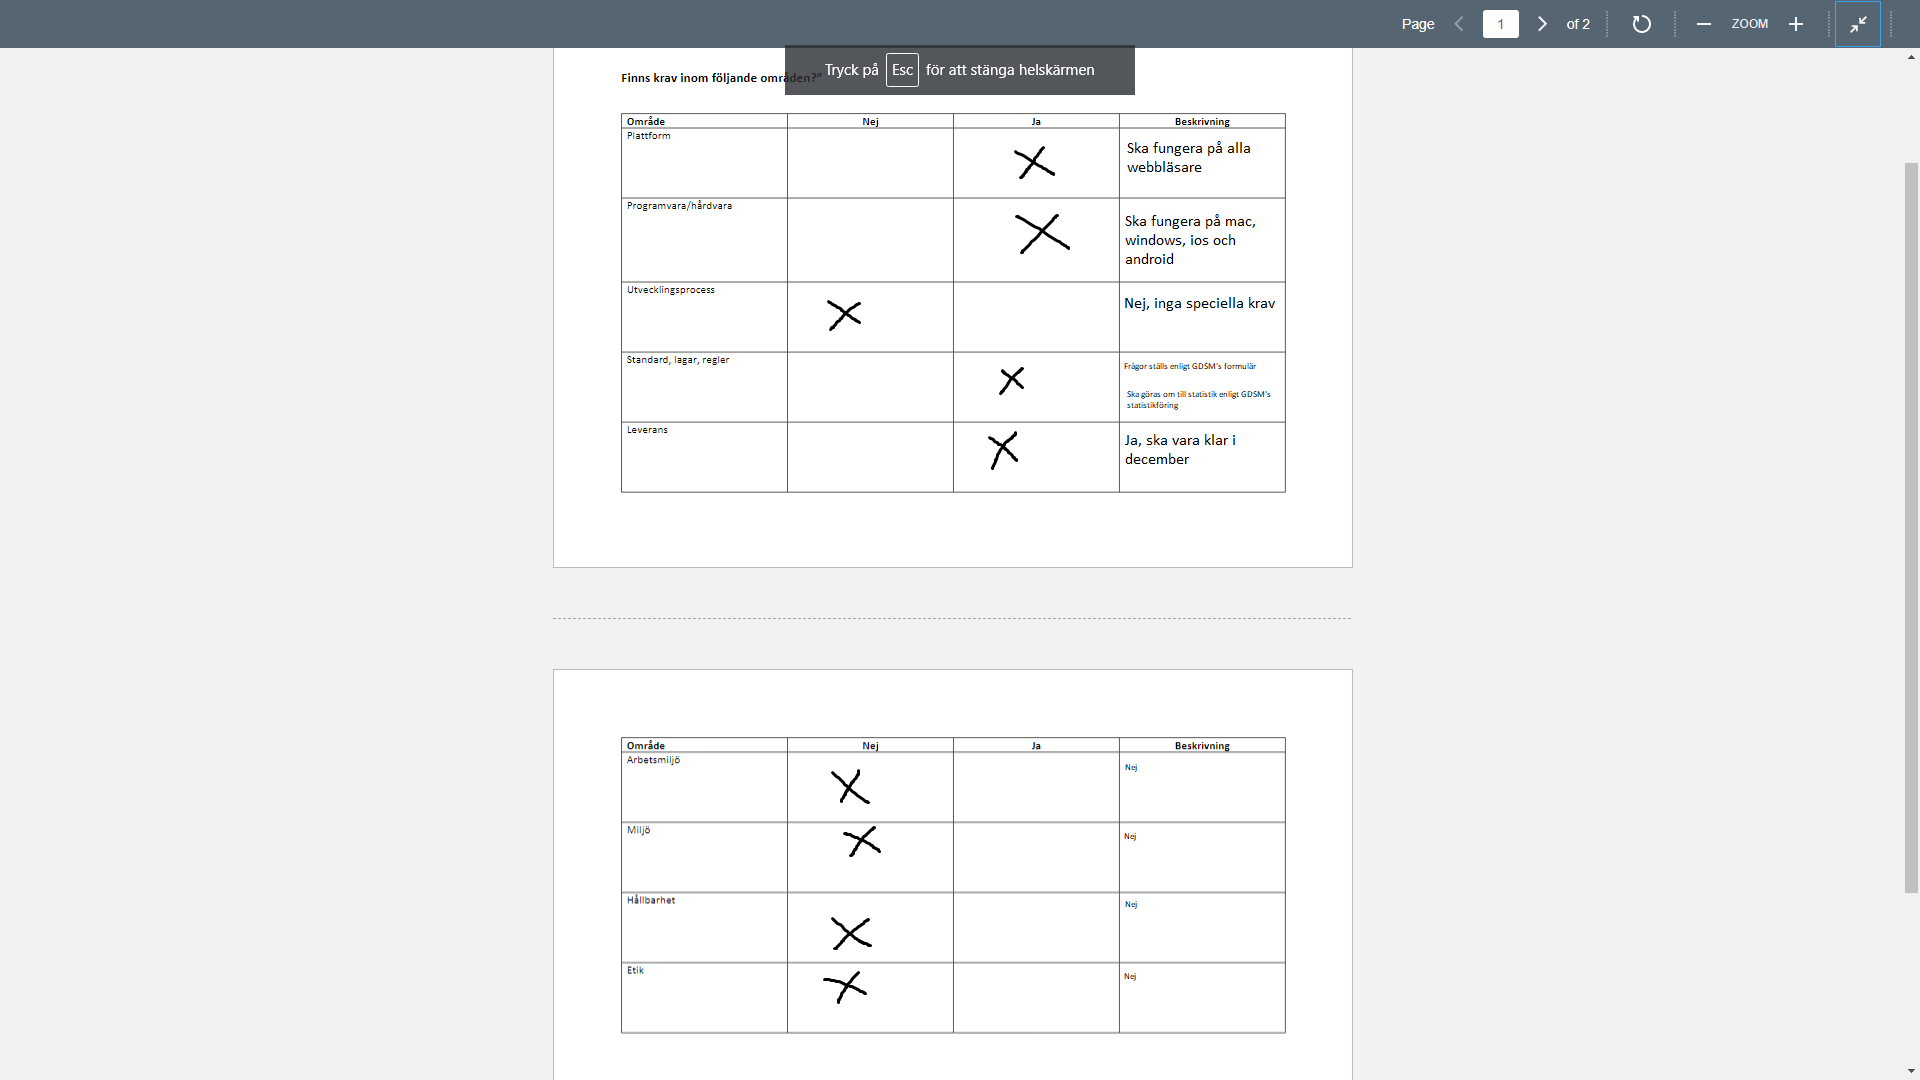
\includegraphics[width = 500px]{24.png}
    \label{fig:24}
\end{figure}
\newpage
\subsection{Kvalitetsfaktorer, kvalitetskrav och risker}

\subsubsection{Kvalitetsfaktorer}
\begin{figure}[htp]
    \centering
    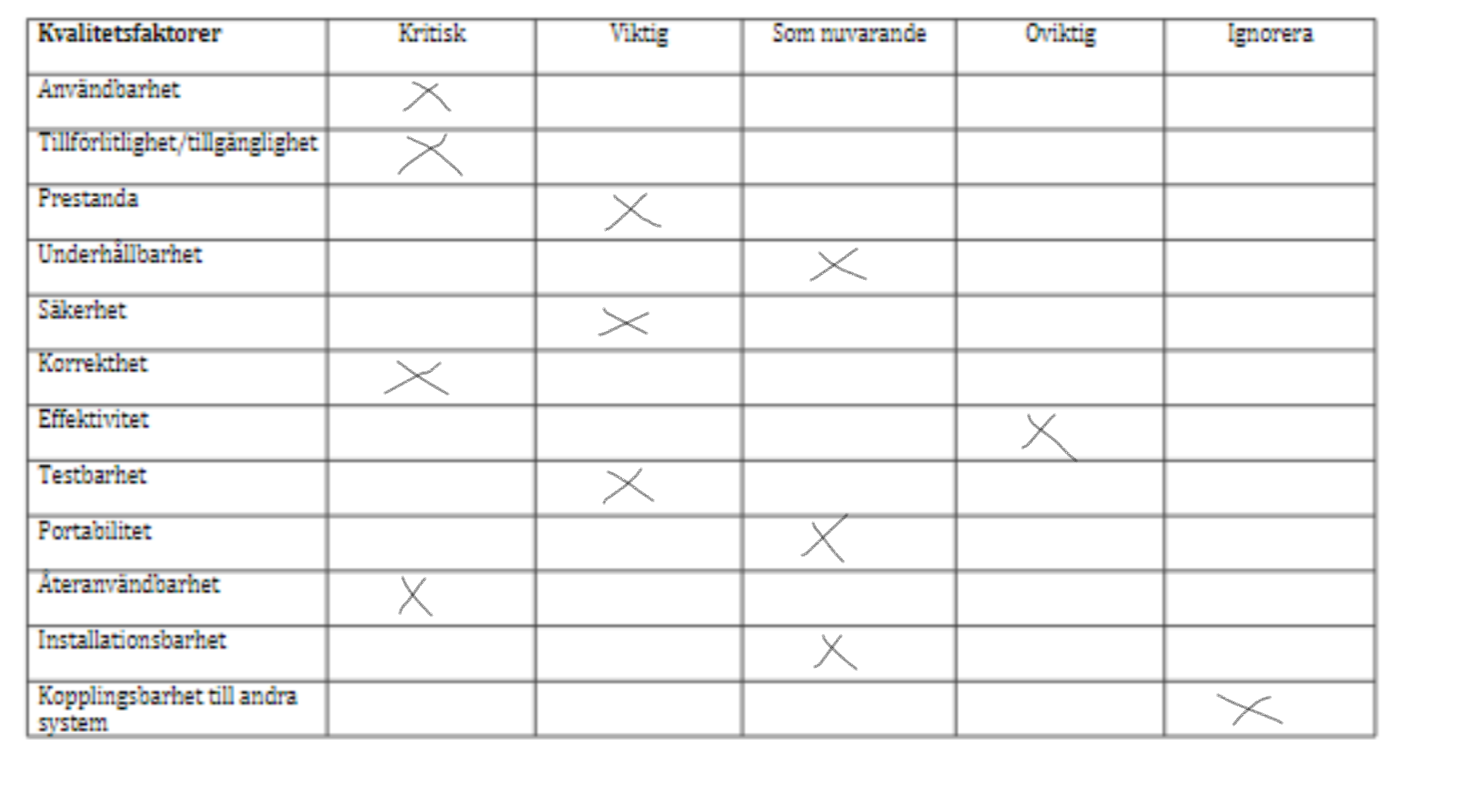
\includegraphics[width = 500px]{41.png}
    \label{fig:24}
\end{figure}




\subsubsection{Kritiska och viktiga kvalitetsfaktorer}

\begin{itemize}

    \item Användbarhet : En lättanvändlig produkt bidrar till att fler användare slutför formuläret vilket ger vår kund bättre statistik. Detta kan i slutändan leda till att kunden får ett stipendium av GDSM
    
     \item Tillgänglighet : Det skall alltid gå att rapportera och extrahera data från verktyget när användaren är uppkopplad till internet. Detta leder till att fler användare kommer kunna rapportera och inte stoppas av möjliga tidskrav, vilket i sin tur leder till bättre statistik och möjligtvis ett stipendium av GDSM
 
     
   \item Prestanda : Sidan ska inte fastna eller hänga sig då detta riskerar att irritera användaren som kan sluta rapportera. En välfungerande sida leder till att fler användare rapporterar in data vilket även detta leder till bättre statistik och möjligtvis ett stipendium av GDSM till kunden.

     \item Säkerhet : Endast behöriga användare ska få tillgång till rapporteringverktyget. Statistiken får inte vara korrupt då detta kan leda till felaktig statistik och ett oanvändbart verktyg.
     
     \item Korrekthet : Statistiken måste stämma överens med verkligheten och får inte bestå av felaktig data då även detta leder till ett oanvändbart verktyg.
     \\
     
     \item Testbarhet : Verktyget måste kunna testas så att kraven kan valideras. Det ska även gå att kolla statistikens korrekthet så att felaktig sammanställning av data inte uppstår.
     
     \item Återanvändbarhet : Kunden vill samla in statistik årligen vilket gör att koden måste kunna återanvändas i samma eller liknande syfte.
     
\end{itemize}

\subsubsection{Kravtext}

\begin{itemize}
    \item  Användbarhet : 95 procent av användarna ska kunna slutföra rapporteringen inom 3 min.
        \item Tillgänglighet : Verktyget ska vara tillgängligt 98 procent av ett år om man har en obesvarad länk.
        \item Tillgänlighet : Verktyget ska vara tillgängligt från iOS, macOS, windows och android. 
    \item Säkerhet : Endast de som har blivit tilldelade en länk via mail ska kunna rappotera data.
    \item Korrekthet : Statistiken ska vara 100 procent korrekt utifrån användarnas rapportering.
    \item Testbarhet :
    \begin{itemize}
        \item [--]Testläge för rapportering ska finnas.
        \item [--]Tester ska ej påverka den slutgiltiga statistiken. 
    \end{itemize}
\end{itemize}

\subsubsection{Riskområden}

\begin{itemize}
    \item Användbarhet : Stora kunskapskillnader hos användare kan leda till att kravet kan vara svårt att säkerhetsställa.
    \begin{description}
          \item[Handlingsplan:] Riskområdet kan ej tas bort helt. Vi kan däremot med utökad testning se till att majoriteten av användarna kan genomföra testet inom kravtiden.
    \end{description}
        \item Tillgänglighet: Oförutsägbara händelser så som strömavbrott och serverfel kan leda till att kravet ej alltid kan uppfyllas. 
        \begin{description}
          \item [Handlingsplan:] Risk kan ej elimineras. För att förminska risken kan vi förlita oss på en pålitlig server samt en backup.
    \end{description}
        \item Tillgänglighet: Gammal mjukvara hos användare kan leda till att alla inte har tillgång till verktyget.
        \begin{description}
          \item[Handlingsplan:] Genom tester och adaptiv programmering kan vi säkerställa att verktyget ser ut och fungerar på samma sätt på så många olika enheter som möjligt.
    \end{description}
   
    \item Säkerhet : Vid ett anfall kan skickliga hackare få tillgång till hemsidan och korrumpera datan.
    \begin{description}
          \item[Handlingsplan:] Kan ej elimineras helt, men genom användning av krypteringsmetoder som SHA-256 samt engångskoder blir påverkan minimal.
    \end{description}
    \item Återanvändbarhet : Då vi endast gör detta som ett skolprojekt är support till kunden inte alltid möjlig.
    \begin{description}
          \item[Handlingsplan:] Kommunicera med kund innan projektets slut för att komma överens om möjlig plan.
    \end{description}
    \item Prestanda : Användaren kan ha dålig hårdvara och/eller uppkoppling. Det kan leda till försämrad användarupplevelse.
    \begin{description}
          \item[Handlingsplan:] Risk kan ej elimineras, men kan minskas genom en optimerad sida.
    \end{description}
    \item Korrekthet : Användaren kan ha dålig uppkoppling vilket kan innebära att användaren har uppfattningen att rapporten är inskickad trots att den inte kommit fram. Leder till förlust av data.
    \begin{description}
          \item[Handlingsplan:] Tydlig kommunikation med användaren om när datan är inskickad och sidan kan stängas ner.
    \end{description}
\end{itemize}

\subsection{Riskanalys enligt miniriskmetoden}
Vi har här använt oss av en metod som kallas miniriskmetoden för att identifiera och analysera risker. Vi tog hjälp av "Riskanalys"[4] för att genomföra denna metod. Det slutade med att vi har kommit fram till ett antal risker och ska nu uppskatta sannolikheten att det sker och konsekvenserna om de sker på en skala 1-4. 
\\

\begin{center}
    \begin{tabular}{|c|c|c|c|c|}
      \hline
      \thead{\makecell{Risk-\\nummer}} & \thead{Projektrisk} & \thead{Sannolikhet} & \thead{Konsekvens} & \thead{Riskmått}\\
      \hline
      2 &\makecell{Dålig uppfattning \\ av tid} & 4 & 4 & 16 \\
      \hline
      5 &\makecell{Konflikter inom \\ gruppen} & 4 & 3 & 12 \\
      \hline
      1 &\makecell{Dålig kommunikation\\ och missförstånd} & 3 & 3 & 9 \\
      \hline
      6 &\makecell{Dålig planering av\\ projektet} & 4 & 2 & 8 \\
      \hline
      9 &\makecell{Försenad information \\ om format på utdata} & 4 & 2 & 8 \\
      \hline
     4 & \makecell{Oförutsägbara händelser} & 2 & 3 & 6 \\
      \hline
      8 & \makecell{Brist på erfarenhet} & 3 & 2 & 6 \\
      \hline
     10 & \makecell{Upptagen kontaktperson,\\innebär långsamma svar} & 2 & 3 & 6 \\
      \hline
     7 & \makecell{Kompetens saknas} & 4 & 1 & 4 \\
      \hline
     3 & \makecell{Förändringar\\i kraven} & 4 & 1 & 4 \\
      \hline
      \end{tabular}
\end{center}
      
      \begin{center}
    \begin{tabular}{|c|c|c|c|c|}
      \hline
      \thead{\makecell{Risk-\\nummer}} & \thead{Produktrisk} & \thead{Sannolikhet} & \thead{Konsekvens} & \thead{Riskmått}\\
       \hline
      2 & \makecell{Produkten är ej \\ tillräckligt intuitiv} & 2 & 4 & 8 \\
      \hline
     4 & \makecell{Bristande javadokumentation} & 4 & 2 & 8 \\
      \hline
      6 & \makecell{För få slutanvändare fyller\\ i formuläret} & 3 & 2 & 6 \\
      \hline
      5 & \makecell{För lite testning} & 3 & 2 & 6 \\
      \hline
      8 &\makecell{Lyckas ej implementera \\ hemsida på server} & 1 & 4 & 4 \\
      \hline
     7 & \makecell{Dåligt val av servertjänst, \\leder till text\\överbelastning } & 1 & 4 & 4 \\
      \hline
     1 & \makecell{Uppfyller ej kraven} & 2 & 2 & 4 \\
      \hline
      9 &\makecell{Produkten är inte \\ tillräckligt säker} & 2 & 2 & 4 \\
      \hline
     3 &\makecell{Dåligt utformad kod} & 3 & 1 & 3 \\
      \hline
     10 & \makecell{Dåliga tester som \\förvränger värdefull\\data} & 1 & 1 & 1 \\
      \hline
    \end{tabular}
\end{center}

\newpage
\subsection{Utvärdering av risker enligt miniriskmetoden}
Här har vi valt de tre  risker med högst riskmått från projket- och produktrisker. Vi har sedan sett vad vi ska vidta för återgärd och vad det förväntade utfallet av återgärden blir. 

 \begin{center}
    \begin{tabular}{ | c | c | c | c |}
      \hline
      \thead{\makecell{Risk-\\nummer}} & \thead{Projektrisk} & \thead{Åtgärd} & \thead{Förväntat utfall} \\
      \hline
      1 & \makecell{Dålig kommunikation\\ och missförstånd} &  \makecell{Tydlig \\ kommunikationsplan \\ samt uppsatta \\ ground roules.}  & \makecell{Bättre stämning och \\ minskad risk för \\missförstånd.} \\
      \hline
      2 & \makecell{Dålig tidsuppfattning} &  \makecell{En god struktur samt \\ kontinuerlig uppföjning \\under sprints.}  & \makecell{Bättre stämning och \\ En bättre uppfattning om \\ projektet ligger i fas.} \\
      \hline
      5 & \makecell{Konflikter inom \\ gruppen} &  \makecell{Respektera varandra, \\ god kommunikartion och, \\ visa förtroende för andra.}  & \makecell{Alla kommer trivas\\ bättre och \\ mer framgångsrikt projekt.} \\
      \hline
       &\makecell{\textbf{Produktrisk}\\} &   &  \\
      \hline
     2 & \makecell{Produkten är ej \\ tillräckligt intuitiv} & Mer användartest.  & \makecell{Bättre helhetsbil\\ av användare} \\
      \hline
       4 &\makecell{Bristande \\ javadokumentation} &\makecell{ Använd javas guide för\\ dokumentation.} & \makecell{Koden blir mer\\ återanvändbar och \\ projektmedlemmarna får \\en större \\ förståelse över koden.} \\
      \hline
      5 & \makecell{För lite testning} & \makecell{Se till att ha en plan över\\ hur ofta och\\ vad man testar.} & \makecell{Med en plan över\\ hur ofta och vad  \\ man tester eliminerar\\ man risken att ha för få tester.} \\
      \hline
    \end{tabular}
  \end{center}


  

\section{Validering och Prioritering}
\subsection {Vilka personer/roller ska läsa kravspecifikationen?}
Christin, samtliga projektmedlemmar, Malin Planander samt Malin Hollgren.
\subsection{Vilken kunskap har dessa om krav?}
Projektmedlemmarna har lekmannamässig kunskap då vi precis påbörjat en kurs inom kravhantering. Somliga har dock erhållit kunskap sedan PUSP-kursen, där en kravspecifikation utformades.\\\\
Malin Hollgren arbetar som projektledare och kan därför förväntas ha kunskap om kravspecifikationer samt kravhantering. Det är hon som i samhötighet med oss utformar kraven efter hennes önskemål och behov. \\\\
Christin är kursledare inom kravhanteringskursen och får därmed anses ha mycket god kunskap. \\\\
Då Malin Planander har varit med vid flera liknande projekt genom åren kan vi anta att hon har god kunskap om hur en kravspecifikation bör skrivas

\subsection{Hur ska kraven specificeras? Dvs hur ska kravspecifikationen byggas upp och se ut?}
Vi har för tillfället valt att börja kategorisera kraven i funktionella-, data och kvalitetskrav. Senare kommer dessa kraven att grupperas utifrån deras områden inom produkten. Till exempel kan datakrav och funktionella krav som berör användarvänlighet grupperas tillsammans.
\begin{enumerate}
    \item För datakraven kommer ER-diagram, virtual windows, kontextdiagram och data dictionary användas.
    \item För de funktionella kraven kommer scenarion användas.
    \item För kvalitetskraven kommer vi använda oss av "open metric and open target" från kurslitteraturen. Dessutom kommer vi använda oss av kapacitets-, pricksäkerhets-, användbarhets-, säkerhets-, support- och prestandakrav
\end{enumerate}

\subsection{Vilka metoder ska användas för att validera kraven i projektet?}

De metoder som kan användas för att validera de krav vi utformar är
\begin{enumerate}
    \item Tester (prototyptester och genomgångar)
    \item Granskningar
\end{enumerate}

\subsection{Hur ska kraven prioriteras?}
I programmet är det viktigt att datan sammanställs korrekt, vilket innebär att dessa kraven är viktigast. Ett av våran mål med arbetet är att så många som möjligt rapporterar in via verktyget, Vilket betyder att även mål om användarvänlighet prioriteras. 

\subsection{Vilka krav ska prioriteras?}
Följande är exempel på krav som ska prioriteras
\begin{enumerate}
    \item 4 av 5 användare ska kunna slutföra rapporteringen inom 3 minuter(open ended metric).
    \item Användare loggar in till formuläret med sin engångskod (scenario).
    \item Datan skall sammanställas på korrekt sätt (enligt GDSMs krav) (data dictionary).
    \item Engångskoden förbrukas när användaren skickar in sin rapport (scenario).
\end{enumerate}
\subsection{Vilken skala ska ni prioritera efter?}
Vi använder oss av: Stabila, ändringsbenägna, uteslutna.
	\item Stabila: Krav som är listade här krävs för att systemet ska definieras som funktionellt.
	\item Ändringsbenägna: Krav som är listade här kan förändras eller tas bort.
	\item Uteslutna: Krav som är listade här är inte längre aktuella
	
\section{Ändringhantering}
Fram till att slutinlämning av kravspecifikationen sker har gruppen bestämt sig för att lägga krav som med stor sannolikhet kommer att ändras under rubriken "Ändringbenägna krav" i kravspecifikationen. Här får även nya krav tillkomma medan borttagna krav kommer läggas under rubriken "Uteslutna krav". När gruppen är säker på att ett krav har fastställts och inte kommer ändras så flyttas kravet till rubriken "Stabila krav". \\
Tillkommer nya krav från kund som inte har ursprung från uppgiftsbeskrivningen kommer gruppen att diskutera detta utifrån två aspekter, kommer det finnas tid för att implementera detta krav? Uppfyller kravet en viktig funktion för produkten?. Anser vi att det kravet är relevant för produkten samt att det finns tid till att genomföra kravet så kommer det att läggas till.  
	
\section{Sammanfattning}´

\subsection{Nyckelintressenter}
Nyckelintressenterna under projektet gång var kunden Malin Hollgren, Malin Planander på miljöbron samt vi i projektgruppen. \\
Med tanke på att Malin Hollgren var den enda kontaktpersonen från Helsingborg Convention & Event Bureau projketgruppen hade så blev hon det enda sättet att säkerhetsställa att projektet var på väg i rätt riktning. Detta var något vi visste i början av projektet och var inget som ändrades. \\
Malin Planander fick däremot mer inflytande över projektet än gruppen tidigare trott. Det visade sig att hon skulle gå från att vara en viktig intressent till att bli en nyckelintressent. Detta på grund av att hon genomgående under projektet styrde upp möten, kom med viktig insikt kring liknande projekt samt gav tips på hur hon tyckte vissa funktioner skulle implementeras.
\\ 

\subsection{Validering av krav}
Gruppen bestämde i tidigt skede att validering av kraven skulle ske genom prototyptester och genomgångar tillsammans med kunden samt interna granskningar inom gruppen. Totalt 3 iterationer där samtliga projektmedlemmar tog fram en egen prototyp och granskades därefter för att se om prototyperna avvek från uppdragsbeskrivningen. Därefter testades prototyperna i intervju med kund. Med hjälp av prototyptesterna och genomgångarna kunde kundens önskemål och behov fastställas mer precist. Den slutgiltiga prototypen uppfyllde de önskemål och behov kunden hade och därmed kunde kraven valideras.\\\\

\subsection{Tre lärdomar kravhanteringen}
Till att börja med anser gruppen att en viktig lärdom var att ha en lätthanterlig prioritering av krav. Under projektet tillkom många krav, speciellt som hade med mindre funktioner inom systemet att göra. Att enkelt kunna lägga till dessa via utan att behöva ändra strukturera om hela dokumentet ledde till en smidigt arbetsprocess.
\\\\
En annan lärdom gruppen har tagit åt sig är att alla projekt är unika och det är upp till gruppen själv att bestämma hur kravhanteringen ska gå till. Det finns många olika delar inom ett projekt som kan påverka detta, hur många kontaktpersoner finns det? Hur tekniskt kunnig är kontaktpersonen? Hur stora är kunden förväntningar? I vårt fall fanns inte all denna information i början av projektet utan det var något som byggdes upp under projektets gång. 
\\\\
Till sist tyckte vi att projektet visade hur viktigt det är med prototyper för att validera krav. Oberoende hur tekniskt kunnig kunden är så anser vi att det är enklast att få fram vad kunden tycker om produkten genom att visa en prototyp. Detta ger ofta feedback i form vad kunden tycker om och vad kunden anser saknas. Det blir en smidigare process för både projektgruppen så som kunden.



\bibliographystyle{alpha}


\end{document}